%%%%%%%%%%%%%%%%%%%%%%%%%%%%%%%%%%%%%%%%%%%%%%%%%%%%%%%%%%%%%%%%%%%%%%
% writeLaTeX Example: A quick guide to LaTeX
%
% Source: Dave Richeson (divisbyzero.com), Dickinson College
% 
% A one-size-fits-all LaTeX cheat sheet. Kept to two pages, so it 
% can be printed (double-sided) on one piece of paper
% 
% Feel free to distribute this example, but please keep the referral
% to divisbyzero.com
% 
%%%%%%%%%%%%%%%%%%%%%%%%%%%%%%%%%%%%%%%%%%%%%%%%%%%%%%%%%%%%%%%%%%%%%%
% How to use writeLaTeX: 
%
% You edit the source code here on the left, and the preview on the
% right shows you the result within a few seconds.
%
% Bookmark this page and share the URL with your co-authors. They can
% edit at the same time!
%
% You can upload figures, bibliographies, custom classes and
% styles using the files menu.
%
% If you're new to LaTeX, the wikibook is a great place to start:
% http://en.wikibooks.org/wiki/LaTeX
%
%%%%%%%%%%%%%%%%%%%%%%%%%%%%%%%%%%%%%%%%%%%%%%%%%%%%%%%%%%%%%%%%%%%%%%

\documentclass[10pt,landscape]{article}
\usepackage{amssymb,amsmath,amsthm,amsfonts}
\usepackage{multicol,multirow}
\usepackage{calc}
\usepackage{ifthen}
\usepackage{physics}
\usepackage{newpxtext,newpxmath}
\usepackage[landscape]{geometry}
\usepackage[colorlinks=true,citecolor=blue,linkcolor=blue]{hyperref}
\usepackage{graphicx}
\usepackage{caption}
\usepackage{empheq}

\DeclareMathOperator*{\argmin}{\arg\!\min}

\ifthenelse{\lengthtest { \paperwidth = 11in}}
    { \geometry{top=.5in,left=.5in,right=.5in,bottom=.5in} }
	{\ifthenelse{ \lengthtest{ \paperwidth = 297mm}}
		{\geometry{top=1cm,left=1cm,right=1cm,bottom=1cm} }
		{\geometry{top=1cm,left=1cm,right=1cm,bottom=1cm} }
	}
\pagestyle{empty}
\newtheorem*{theorem*}{Theorem}
\newtheorem*{definition*}{Definition}
\newtheorem*{example*}{Example}
\makeatletter
\renewcommand{\section}{\@startsection{section}{1}{0mm}%
                                {-1ex plus -.5ex minus -.2ex}%
                                {0.5ex plus .2ex}%x
                                {\normalfont\large\bfseries}}
\renewcommand{\subsection}{\@startsection{subsection}{2}{0mm}%
                                {-1explus -.5ex minus -.2ex}%
                                {0.5ex plus .2ex}%
                                {\normalfont\normalsize\bfseries}}
\renewcommand{\subsubsection}{\@startsection{subsubsection}{3}{0mm}%
                                {-1ex plus -.5ex minus -.2ex}%
                                {1ex plus .2ex}%
                                {\normalfont\small\bfseries}}
\makeatother
\setcounter{secnumdepth}{0}
\setlength{\parindent}{0pt}
\setlength{\parskip}{0pt plus 0.5ex}

\newcommand*\widefbox[1]{\fbox{\hspace{2em}#1\hspace{2em}}}
% -----------------------------------------------------------------------

\title{Quick Guide to LaTeX}

\begin{document}

\raggedright
\footnotesize

\begin{center}
     \Large{\textbf{Machine Learning (ML)}} \\
\end{center}
\begin{multicols}{3}
\setlength{\premulticols}{1pt}
\setlength{\postmulticols}{1pt}
\setlength{\multicolsep}{1pt}
\setlength{\columnsep}{2pt}

\section{Prerequisites}

\begin{definition*}[\textbf{Real Vector Space}]
A set $\mathcal{H}$ is called a vector space over $\mathbb{R}$ if addition and scalar multiplication are defined, and satisfy $\forall \mathbf{x}, \mathbf{x'}, \mathbf{x''} \in \mathcal{H}$ and $\lambda, \lambda' \in \mathbb{R}$:
\begin{align*}
& \mathbf{x} + \left( \mathbf{x'} + \mathbf{x''} \right) = \left( \mathbf{x} + \mathbf{x'} \right) + \mathbf{x''}, \\
& \mathbf{x} + \mathbf{x'} = \mathbf{x'} + \mathbf{x} \in \mathcal{H}, \\ 
& 0 \in \mathcal{H}, \mathbf{x} + 0 = \mathbf{x}, \\ 
& -\mathbf{x} \in \mathcal{H}, \mathbf{x} - \mathbf{x} = 0, \\ 
& \lambda \mathbf{x} \in \mathcal{H}, \\
& 1 \mathbf{x} \in \mathcal{H}, \\
& \lambda \left( \lambda' \mathbf{x} \right) = \left( \lambda \lambda' \right) \mathbf{x}, \\
& \lambda \left( \mathbf{x} + \mathbf{x'} \right) = \lambda \mathbf{x} + \lambda \mathbf{x'} \\
\end{align*}
\end{definition*}

\begin{definition*}[\textbf{Norm}]
A function $\Vert \cdot \Vert : \mathcal{H} \rightarrow \mathbb{R}_0^{+}$ that for all $\mathbf{x}, \mathbf{x'} \in \mathcal{H}$ and $\lambda \in \mathbb{R}$ satisfies:
\begin{align*}
& \Vert \mathbf{x} + \mathbf{x'} \Vert \leq \Vert \mathbf{x} \Vert + \Vert \mathbf{x'} \Vert, \\
& \Vert \lambda \mathbf{x} \Vert = \vert \lambda \vert \Vert \mathbf{x} \Vert, \\
& \Vert \mathbf{x} \Vert > 0 \textrm{ if } \mathbf{x} \neq 0,
\end{align*}
is called a norm on $\mathcal{H}$.
\end{definition*}

\begin{definition*}[\textbf{Dot Product}]
A dot product on a vector space $\mathcal{H}$ is a symmetric bilinear form,
\begin{align*}
\langle ., . \rangle : \mathcal{H} \times \mathcal{H} & \rightarrow \mathbb{R} \\
\left( \mathbf{x}, \mathbf{x'} \right) & \mapsto \langle \mathbf{x}, \mathbf{x'} \rangle
\end{align*}
that is strictly positive definite.
\end{definition*}

\begin{definition*}[\textbf{Normed Space and Dot Product Space}]
A normed space is a vector space endowed with a norm; a dot product space (pre-Hilbert space) is a vector space endowed with a dot product.
\end{definition*}

\begin{definition*}[\textbf{Cauchy Sequence}]
A sequence $\left( \mathbf{x}_i \right)_i \coloneq \left( \mathbf{x}_i \right)_{i \in \mathbb{N}} = \left( \mathbf{x}_1, \mathbf{x}_2, \dots \right)$ in a normed space $\mathcal{H}$ is said to be a Cauchy sequence if for every $\epsilon > 0$, there exists an $n \in \mathbb{N}$ such that for all $n', n'' > n$, $\Vert \mathbf{x}_{n'} - \mathbf{x}_{n''} \Vert < \epsilon$.
\end{definition*}

\begin{definition*}[\textbf{Hilbert Space}]
A space $\mathcal{H}$ is called complete if all Cauchy sequences in the space converge. A Hilbert space is a complete dot product space. Hilbert spaces have infinite dimensionality.
\end{definition*}

\begin{example*}[\textbf{Hilbert Space of  Functions}]
Let $C\left[a, b\right]$ denote the real-valued continuous functions on the interval $\left[a, b\right]$ For $f, g \in C\left[a, b\right]$,
\begin{equation*}
\langle f, g \rangle \coloneq \int_{a}^{b} f(x)g(x) dx
\end{equation*}
defines a dot product. The completion of $C\left[a, b\right]$ in the corresponding norm is the Hilbert space $L_2 \left[a, b\right]$ of measurable functions that are square integrable:
\begin{equation*}
\int_{a}^{b} f^2(x) dx < \infty
\end{equation*}
\end{example*}

\section{Elements of Statistical Learning Theory}

\subsection{Learning problem}

In two-class pattern recognition, we seek to infer a function:

\begin{equation*}
f : \mathcal{X} \rightarrow \left\lbrace \pm 1 \right\rbrace
\end{equation*}

Statistical learning theory makes the assumption that the data are generated by sampling from an unknown underlying distribtuion $P(x,y)$. The learning problem then consists in minimizing the \textit{risk}:

\begin{equation*}
R \left[ f \right] = \int_{\mathcal{X} \times \mathcal{Y}} \underbrace{c\left(x,y,f(x)\right)}_{\textrm{loss function}} dP(x,y)
\end{equation*}

We do not know $P$. We do know the training data, which are sample from $P$. This leads to the empirical risk:

\begin{equation*}
R_{emp} \left[ f \right] = \frac{1}{m}\sum_{i=1}^{m} c(x_i,y_i,f(x_i))
\end{equation*}

For the purpose of bounding the probability:
\begin{equation*}
P \left\lbrace \sup_{f \in \mathcal{F}} \left( R \left[ f \right] - R_{emp} \left[ f \right] \right) > \epsilon \right\rbrace
\end{equation*}

The function class $\mathcal{F}$ is effectively finite. Let $Z_{2m} \coloneqq \left( \left( x_1, y_1 \right), \dots, \left(x_{2m}, y_{2m} \right) \right)$ be the given $2m$-sample. Denote by $\mathcal{N} \left( \mathcal{F}, Z_{2m} \right)$ the cardinality of $\mathcal{F}$ when restricted to $\left\lbrace x_1, \dots, x_{2m} \right\rbrace$, that is, the number of functions from $\mathcal{F}$ that can be distinguished from their values on $\left\lbrace x_1, \dots, x_{2m} \right\rbrace$. Denote the maximum number of functions that can be distinguished as $\mathcal{N} \left( \mathcal{F}, 2m \right)$. The function $\mathcal{N} \left( \mathcal{F}, m \right)$ is referred to as the \textit{shattering coefficient}. It measures the number of ways that the function class can separate the patterns into two classes. 

\subsubsection{VC Dimension and Other Capacity Concepts}

By taking a supremum over all possible samples:

\begin{equation*}
G_{\mathcal{F}} (m) = \max_{(x_1,y_1),\dots,(x_m,y_m) \in \mathcal{X} \times \left\lbrace \pm \right\rbrace} \ln \mathcal{N} \left( \mathcal{F}, (x_1,y_1),\dots,(x_m,y_m) \right)
\end{equation*}

this leads to the \textit{growth function}. If $\mathcal{F}$ is as rich as possible, so that for any sample of size $m$, they can be separated in all $2^m$ possible ways (i.e., they can be shattered), then:

\begin{equation*}
G_{\mathcal{F}} (m) = m \cdot \ln(2)
\end{equation*}

There exists some \textit{maximal} $m$ for which it is satisfied (\textit{VC dimension}). The VC dimension can be shown to be $N+1$ for hyperplanes in $\mathbb{R}^N$.

\subsection{Linear regression}

Method for predicting a real-valued output (also called the \textbf{dependent variable} or \textbf{target}) $y \in \mathbb{R}$ given a vector of real-valued inputs (also called \textbf{independent variables, explanatory variables} or \textbf{covariates}) $\mathbf{x} \in \mathbb{R}^D$.

Linear regression usually refers to a model of the form:

\begin{equation*}
p\left( y \mid \mathbf{x}, \mathbf{\theta} \right) = \mathcal{N}\left( y \mid \mathbf{w}^T \mathbf{x}+b, \sigma^2 \right)
\end{equation*}

where $\mathbf{\theta} = \left( b, \mathbf{w}, \sigma^2 \right)$ are the parameters. The \textbf{residual sum of squares} is given by:

\begin{equation*}
\frac{1}{2} \sum_{n=1}^{N} \left( y_n - \mathbf{w}^T \mathbf{x}_n \right)^2 = \frac{1}{2} \Vert \mathbf{X}\mathbf{w}-\mathbf{y}\Vert^2 = \frac{1}{2} \left( \mathbf{X}\mathbf{w}-\mathbf{y} \right)^T \left( \mathbf{X}\mathbf{w}-\mathbf{y} \right)
\end{equation*}
Setting the gradient to zero and solving gives:
\begin{align*}
& \nabla_{\mathbf{w}} \left( \frac{1}{2} \left( \mathbf{X}\mathbf{w}-\mathbf{y} \right)^T \left( \mathbf{X}\mathbf{w}-\mathbf{y} \right) \right) = & \\
& \nabla_{\mathbf{w}} \left( \mathbf{w}^T \mathbf{X}^T \mathbf{X} \mathbf{w} - \mathbf{w}^T \mathbf{X}^T \mathbf{y} - \mathbf{y}^T \mathbf{X} \mathbf{w} + \mathbf{y}^T\mathbf{y} \right) = & \\
& \nabla_{\mathbf{w}} \left( \mathbf{w}^T \mathbf{X}^T \mathbf{X} \mathbf{w} -  2 \mathbf{w}^T\mathbf{X}^T\mathbf{y} + \mathbf{y}^T\mathbf{y} \right) = & \\
& 2 \mathbf{X}^T \mathbf{X} \mathbf{w} - 2 \mathbf{X}^T\mathbf{y} = 0 & \\
& \boxed{\hat{\mathbf{w}} = \left( \mathbf{X}^T \mathbf{X} \right)^{-1} \mathbf{X}^T\mathbf{y}}
\end{align*}

\subsection{Ridge regression/$l_2$ regularization/Tikhonov regularization}

Maximum likelihood estimation can result in overfitting. The main solution to overfitting is to use \textbf{regularization}, which means to add a penalty term to the empirical risk. Thus we optimize:

\begin{align*}
& \boxed{\hat{\mathbf{w}}_{map} = \argmin \frac{1}{2} \left( \mathbf{X}\mathbf{w}-\mathbf{y} \right)^T \left( \mathbf{X}\mathbf{w}-\mathbf{y} \right) + \lambda \Vert \mathbf{w} \Vert^2} \\
& \boxed{\hat{\mathbf{w}}_{map} = \left( \mathbf{X}^T \mathbf{X} + \lambda \mathbf{I} \right)^{-1} \mathbf{X}^T\mathbf{y}}
\end{align*}

\subsubsection{Feature extraction}
In general, a straight line will not provide a good fit. We can always apply a nonlinear transformation to the input features by replacing $\mathbf{x}$ with $\phi\left(\mathbf{x}\right)$. For example, we can use a polynomial transform, which in 1D is given by $\phi \left( x \right) = \left[ 1, x, x^2, x^3, \dots \right]$. The model becomes:

\begin{equation*}
\boxed{f \left( \mathbf{x}; \mathbf{\theta} \right) = \mathbf{W}\phi \left( \mathbf{x} \right) + \mathbf{b}}
\end{equation*}

\section{Support vector machines (SVMs)}

Consider a \textbf{binary classifier} of the form  $h(\mathbf{x})=\textrm{sign}\left(f(\mathbf{x})\right)$ where the decision boundary is given by:

\begin{equation*}
f(\mathbf{x}) = \mathbf{w}^{T}\mathbf{x} + b
\end{equation*}

Labels are -1 and +1 rather than 0 and 1.

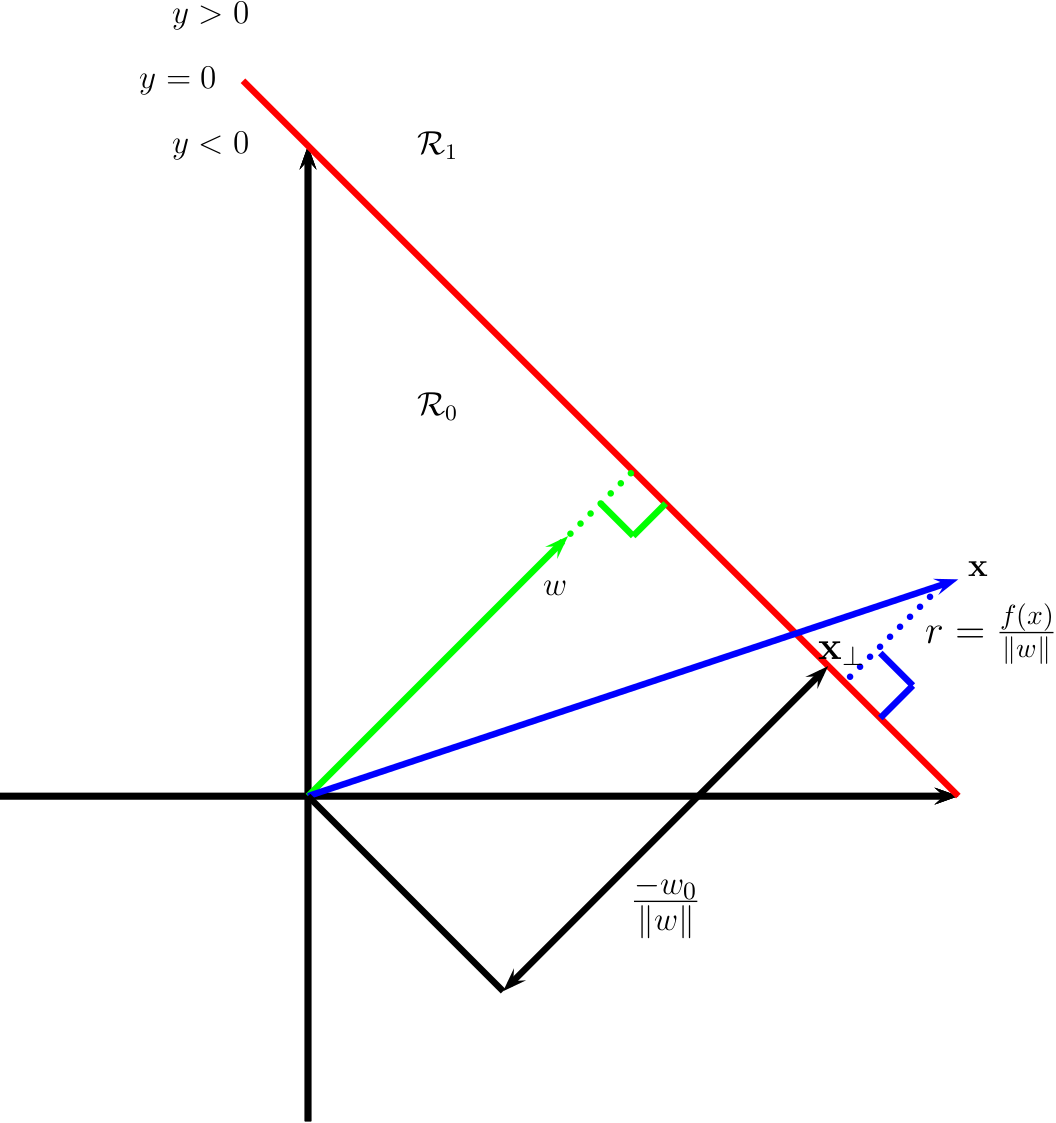
\includegraphics[width=0.25\textwidth]{Figure_17.13_A.png}

The distance of a point to the decision boundary is:

\begin{equation*}
\mathbf{x} = \mathbf{x}_{\bot} + r\frac{\mathbf{w}}{\Vert \mathbf{w} \Vert}
\end{equation*}

where $r$ is the distance of $\mathbf{x}$ from the decision boundary whose normal vector is $\mathbf{w}$, and $\mathbf{x}_{\bot}$ is the orthogonal projection of $\mathbf{x}$ onto this boundary.

\begin{definition*}
\textbf{(Geometrical Margin)} For a hyperplane $\left\lbrace \mathbf{x} \in \mathcal{H} \mid \langle\mathbf{w}, \mathbf{x}\rangle + b = 0 \right\rbrace$, we call
\begin{equation*}
\rho_{(\mathbf{w}, b)} (\mathbf{x}, y) \coloneqq y \left( \langle \mathbf{w}, \mathbf{x} \rangle + b \right)/ \Vert \mathbf{w} \Vert
\end{equation*}
the geometrical margin of the point $(\mathbf{x},y) \in \mathcal{H} \times \lbrace \pm 1 \rbrace$. The minimum value 
\begin{equation*}
\rho_{(\mathbf{w}, b)} \coloneqq \min_{i=1,\dots,m} \rho_{(\mathbf{w}, b)} (\mathbf{x}_i, y_i)
\end{equation*}
shall be called the geometrical margin of $(\mathbf{x}_1, y_1), \dots, (\mathbf{x}_m, y_m)$.
\end{definition*}


\begin{align*}
f(\mathbf{x}) & = \mathbf{w}^{T}\mathbf{x} + b \\
& = \mathbf{w}^{T}\mathbf{x}_{\bot}+b+r\frac{\mathbf{w}^{T}\mathbf{w}}{\Vert \mathbf{w} \Vert} \\
& = \mathbf{w}^{T}\mathbf{x}_{\bot}+b+r{\Vert \mathbf{w} \Vert}
\end{align*}

Since $0 = f(\mathbf{x}_{\bot}) = \mathbf{w}^{T}\mathbf{x}_{\bot}+b$, we have $f(\mathbf{x}) = r{\Vert \mathbf{w} \Vert}$ and hence $r=\frac{f(\mathbf{x})}{\Vert \mathbf{w} \Vert}$. We also require $f(\mathbf{x}_n)y_n > 0$ (ensure each point is on the correct side of the boundary). We want:

\begin{equation*}
\underbrace{\max_{\mathbf{w}, b} \frac{1}{\Vert \mathbf{w} \Vert}}_{\textrm{maximize the distance}} \underbrace{\min_{n=1}^{N} \left[ y_n\left( \mathbf{w}^{T}\mathbf{x}_n+b\right) \right]}_{\textrm{of the closest point}}
\end{equation*}

Let us define the scale factor such that $y_n f_n = 1$ for the point that is closest to the decision boundary. Hence we require $y_n f_n \geq 1$ for all $n$. Maximizing $1/\Vert \mathbf{w} \Vert$ is equivalent to minimizing $\Vert \mathbf{w} \Vert^2$. Thus:

\begin{equation*}
\boxed{\min_{\mathbf{w}, b}\frac{1}{2}\Vert \mathbf{w} \Vert^2 \quad \textrm{s.t. } y_n\left( \mathbf{w}^{T}\mathbf{x}_n + b \right) \geq 1}
\end{equation*}

$N+D+1$ variables subject to $N$ constraints (\textbf{primal problem}).

In convex optimization, for every primal problem we can derive a \textbf{dual problem}. Let $\mathbf{\alpha} \in \mathbb{R}^N$ be the dual variables corresponding to Lagrange multipliers that enforce $N$ inequality constraints:

\begin{equation*}
\mathcal{L}\left( \mathbf{w}, b, \mathbf{\alpha}\right) = \frac{1}{2}\mathbf{w}^T\mathbf{w}-\sum_{n=1}^N \alpha_n \left( y_n \left( \mathbf{w}^{T}\mathbf{x}_n + b \right) - 1 \right)
\end{equation*}

We have:

\begin{align*}
& \nabla_{\mathbf{w}} \mathcal{L}\left( \mathbf{w}, b, \mathbf{\alpha}\right) = \mathbf{w} - \sum_{n=1}^N \alpha_n y_n\mathbf{x}_n \\
& \frac{\partial}{\partial b} \mathcal{L}\left( \mathbf{w}, b, \mathbf{\alpha}\right) = - \sum_{n=1}^N \alpha_n y_n
\end{align*}

and hence:

\begin{align*}
& \hat{\mathbf{w}} = \sum_{n=1}^N \hat{\alpha}_n y_n\mathbf{x}_n \\
& 0 = \sum_{n=1}^N \hat{\alpha}_n y_n
\end{align*}

Plugging these into the Lagrangian:

\begin{align*}
\mathcal{L}\left( \hat{\mathbf{w}}, \hat{b}, \mathbf{\alpha}\right) & = \frac{1}{2}\hat{\mathbf{w}}^T\hat{\mathbf{w}}-\sum_{n=1}^N \alpha_n y_n \hat{\mathbf{w}}^{T}\mathbf{x}_n - \sum_{n=1}^N \alpha_n y_n \hat{b} + \sum_{n=1}^N \alpha_n \\
& = \frac{1}{2}\hat{\mathbf{w}}^T\hat{\mathbf{w}} - \hat{\mathbf{w}}^T\hat{\mathbf{w}} - 0 + \sum_{n=1}^N \alpha_n \\
& = \boxed{- \frac{1}{2} \sum_{i=1}^{N} \sum_{j=1}^{N} \alpha_i \alpha_j y_i y_j \mathbf{x}_i^{T} \mathbf{x}_j + \sum_{n=1}^N \alpha_n}
\end{align*}

We want to maximize this wrt $\mathbf{\alpha}$ subject to the constraints $\sum_{n=1}^N \alpha_n y_n = 0$ and $\alpha_n \geq 0$ ($N$ variables).

KKT conditions:

\begin{align*}
\alpha_n & \geq 0 \\
y_n f(\mathbf{x}) - 1 & \geq 0 \\
\alpha_n \left( y_n f(\mathbf{x}) - 1 \right) & \geq 0
\end{align*}

Hence either $\alpha_n = 0$ or $y_n \left( \hat{\mathbf{w}}^T \mathbf{x}_n + \hat{b} \right) = 1$ is active (sample $n$ lies on the decision boundary; \textbf{support vector}).

Denote by $\mathcal{S}$ the set of support vectors. To perform prediction:

\begin{equation*}
\boxed{f ( \mathbf{x}; \hat{\mathbf{w}}, \hat{b} ) = \hat{\mathbf{w}}^T \mathbf{x} + b = \sum_{n \in \mathcal{S}} \alpha_n y_n \mathbf{x}_n^{T}\mathbf{x} + b}
\end{equation*}

\subsubsection{Soft margin classifiers}

If data is not linearly separable, there will be no feasible solution in which $y_n f_n \geq 1$ for all $n$. We therefore introduce \textbf{slack variables} $\xi_n \geq 0$ and replace the hard constraints $y_n f_n \geq 0$ with $y_n f_n \geq 1 - \xi_n$. The new objective becomes:

\begin{equation*}
\boxed{\min_{\mathbf{w}, b, \mathbf{\xi}}\frac{1}{2}\Vert \mathbf{w} \Vert^2 + C\sum_{n=1}^{N} \xi_n \quad \textrm{s.t. } \xi_n \geq 0, y_n\left( \mathbf{w}^{T}\mathbf{x}_n + b \right) \geq 1 - \xi_n}
\end{equation*}

$C$ is a hyperparameter controlling how many points violate the margin constraints (if $C = \infty$ we recover the unregularized, hard-margin classifier).

The corresponding Lagrangian for the soft margin classifier becomes:

\begin{align*}
\mathcal{L}\left( \mathbf{w}, b, \mathbf{\alpha}, \mathbf{\xi}, \mathbf{\mu} \right) & = \frac{1}{2}\mathbf{w}^T\mathbf{w} + C\sum_{n=1}^N \xi_n - \\
& \sum_{n=1}^N \alpha_n \left( y_n \left( \mathbf{w}^{T}\mathbf{x}_n + b \right) - 1 + \xi_n \right) - \sum_{n=1}^{N} \mu_n \xi_n
\end{align*}

where $\alpha_n \geq 0$ and $\mu_n \geq 0$ are the Lagrange multipliers. Optimizing out $\mathbf{w}$, $b$ and $\mathbf{\xi}$ gives the dual form identical to the hard margin case. However, the KKT conditions imply:

\begin{align*}
0 \leq \alpha_n \leq C \\
\sum_{n=1}^{N} \alpha_n y_n = 0
\end{align*}

If $\alpha_n = 0$, the point is ignored.

If $0 < \alpha_n < C$, then $\xi_n = 0$, so the point lies on the margin.

If $\alpha_n = C$, the point can either be correctly classified if $\xi_n \leq 1$, or misclassified if $\xi_n > 1$. Hence $\sum_n \xi_n$ is an upper bound on the number of misclassified points.

\begin{center}
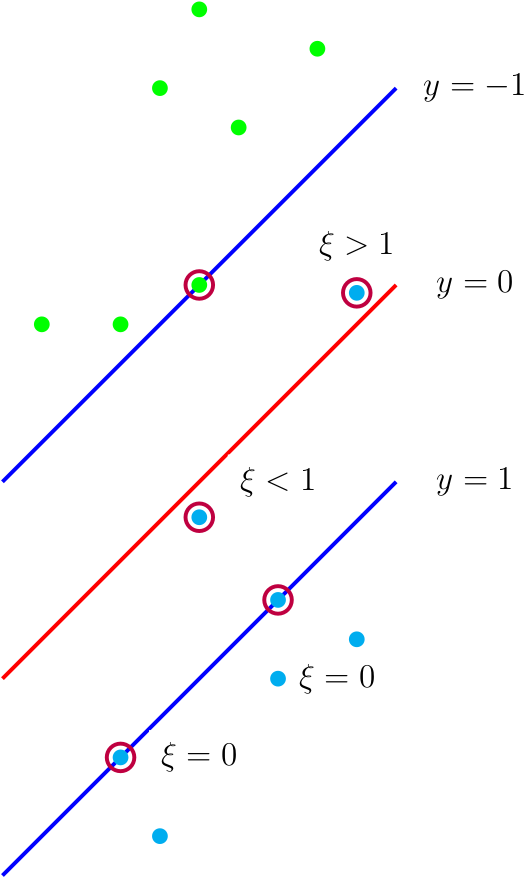
\includegraphics[width=0.1\textwidth]{Figure_17.13_B.png}
\end{center}

\subsection*{Kernels}

\subsubsection{Kernel trick}
The principal benefit of the dual problem is that we can replace all inner product operations $\mathbf{x}^{T}\mathbf{x'}$ with a call to a positive definite kernel function $\mathcal{K}(\mathbf{x}, \mathbf{x'})$. The kernel trick allows us to avoid having to deal with an explicit feature representation of our data. In particular:
\begin{equation*}
f(\mathbf{x}) = \hat{\mathbf{w}}^{T}\mathbf{x}+b = \sum_{n \in \mathcal{S}} \alpha_n y_n \mathbf{x}_n^{T}\mathbf{x} + \hat{b} = \sum_{n \in \mathcal{S}} \alpha_n y_n \mathcal{K}(\mathbf{x}_n, \mathbf{x'}) + \hat{b}
\end{equation*}

\fbox{%
    \parbox{0.315\textwidth}{A simple type of similarity measure is a \textit{dot product}. For instance, given two vectors $\mathbf{x}, \mathbf{x'} \in \mathbb{R}^{N}$, the canonical dot product is defined as:

\begin{equation*}
\langle \mathbf{x}, \mathbf{x'} \rangle \coloneqq \sum_{i=1}^{N} [\mathbf{x}]_i[\mathbf{x'}]_i
\end{equation*}

Patterns could be any kind of object. In order to be able to use a dot product as a similarity measure, we therefore first need to represent the patterns as vectors in some dot product space $\mathcal{H}$:

\begin{align*}
\mathbf{\Phi} : \mathcal{X} & \rightarrow \mathcal{H} \\
x & \mapsto \mathbf{x} \coloneqq \mathbf{\Phi}(x)
\end{align*}

The space $\mathcal{H}$ is called a \textit{feature space}. A similarity measure from the dot product in $\mathcal{H}$:

\begin{equation*}
k(x,x') \coloneqq \langle \mathbf{x}, \mathbf{x'} \rangle = \langle \mathbf{\Phi}(x), \mathbf{\Phi}(x') \rangle
\end{equation*}

In binary classification, two labels (outputs) can either be identical or different. Let us consider a similarity measure of the form:

\begin{align*}
k : \mathcal{X} \times \mathcal{X} & \rightarrow \mathbb{R} \\
(x, x') & \mapsto k(x,x')
\end{align*}

that is, a function that given two patterns returns a real number characterizing their similarity.}}


\subsubsection*{Product Features}

For $\mathcal{X}$ a subset of the vector space $\mathbb{R}^N$, $N = d = 2$, dot products in $\mathcal{H}$ for the map:
\begin{equation*}
\mathbf{\Phi} : \left( \left[x\right]_1, \left[x\right]_2 \right) \mapsto \left( \left[x\right]_1^2, \left[x\right]_2^2, \left[x\right]_1\left[x\right]_2, \left[x\right]_2\left[x\right]_1\right)
\end{equation*}
take the form:
\begin{equation*}
\langle \mathbf{\Phi}(x), \mathbf{\Phi}(\mathit{x'}) \rangle = \left[x\right]_1^2\left[\mathit{x'}\right]_1^2 + \left[x\right]_2^2\left[\mathit{x'}\right]_2^2 + 2\left[x\right]_1\left[x\right]_2\left[\mathit{x'}\right]_1\left[\mathit{x'}\right]_2 = \langle x, x' \rangle^2
\end{equation*}
In other words, the desired kernel is simply the square of the dot product in input space. The same works for arbitrary $N,d\in \mathbb{N}$.

\subsubsection*{Positive Definite Kernels}
The results in this section hold for data drawn from domains which need no structure.
\begin{definition*}
\textbf{(Gram Matrix)} Given a function $k : \mathcal{X}^2 \rightarrow \mathbb{R}$ and patterns $x_1, \dots, x_m \in \mathcal{X}$, the  $m \times m$ matrix $K$ with elements $K_{ij} \coloneq k(x_i, x_j)$ is called the Gram matrix of $k$.
\end{definition*}

\begin{definition*}
\textbf{(Positive Definite Matrix)} A real symmetric\footnote{$k(x_i, x_j) = k(x_j, x_i)$} $m \times m$ matrix $K$ satisfying $\sum_{i,j} c_i c_j K_{ij} \geq 0$ for all $c_i \in \mathbb{R}$ is called positive definite.
\end{definition*}

\begin{definition*}
\textbf{(Positive Definite Kernel)} A function $k$ on $\mathcal{X} \times \mathcal{X}$ gives rise to positive definite Gram matrix is called a positive definite kernel.
\end{definition*}

\subsubsection*{The Reproducing Kernel Map}
We describe the construction of a dot product on the function space such that $k(x,x')=\langle \mathbf{\Phi}(x), \mathbf{\Phi}(x')\rangle$. Here $\mathbf{\Phi}(x)$ denotes the function that assigns the value $k(x',x)$ to $x' \in \mathcal{X}$, i.e., $\mathbf{\Phi}(x)(\cdot) = k(\cdot,x)$.

We define a vector space by taking linear combinations of the form:
\begin{equation*}
f(\cdot) = \sum_{i=1}^{m} \alpha_i k \left( \cdot, x_i \right)
\end{equation*}

Here, $m \in \mathbb{N}$, $\alpha_i \in \mathbb{R}$ and $x_1, \dots, x_m \in \mathcal{X}$ are arbitrary.

Next, we define a dot product between $f$ and another function:
\begin{equation*}
g(\cdot) = \sum_{j=1}^{m'} \beta_j k \left( \cdot, x_j^{'} \right)
\end{equation*}

as:
\begin{equation*}
\langle f, g \rangle = \sum_{i=1}^{m}\sum_{j=1}^{m'} \alpha_i \beta_j k \left( x_i, x_j^{'} \right) \stackrel{\textrm{sym.}}{=} \langle g, f \rangle
\end{equation*}

Moreover,
\begin{equation*}
\langle f, f \rangle = \sum_{i, j=1}^{m}\alpha_i \alpha_j k \left( x_i, x_j \right) \stackrel{\textrm{pd}}{\geq} 0
\end{equation*}

In proving that it qualifies as a dot product:
\begin{equation*}
\langle k(\cdot, x), f \rangle = f(x)
\end{equation*}

In particular:
\begin{equation*}
\langle k(\cdot, x), k(\cdot, x') \rangle = k(x, x')
\end{equation*}

By virtue of these properties, pd kernels are also called \textit{reproducting kernels}. The above reasoning has shown that any positive definite kernel can be thought as a dot product in another space. In view of:
\begin{align*}
k : \mathcal{X} \times \mathcal{X} & \rightarrow \mathbb{R} \\
(x, x') & \mapsto k(x,x')
\end{align*}
the reproducing kernel property:
\begin{equation*}
\langle k(\cdot, x), k(\cdot, x') \rangle = k(x, x')
\end{equation*}
amounts to:
\begin{equation*}
\langle \mathbf{\Phi}(x), \mathbf{\Phi}(x') \rangle = k(x, x')
\end{equation*}

\subsubsection*{Reproducing Kernel Hilbert Spaces}
\begin{definition*}[\textbf{Reproducing Kernel Hilbert Space}]
$\mathcal{H}$ is called a reproducing kernel Hilbert space endowed with the dot product and the norm ($\Vert f \Vert \coloneq \sqrt{\langle f,f\rangle}$) if there exists a function $k : \mathcal{X} \times \mathcal{X} \rightarrow \mathbb{R}$ with the following properties:
\begin{enumerate}
\item (Reproducing Property) $k$ has the reproducing property
\begin{equation*}
\langle f, k(x, \cdot) \rangle = f(x) \quad \textrm{for all } f \in \mathcal{H}
\end{equation*}
\item (Closed Space) $k$ spans $\mathcal{H}$, i.e., $\mathcal{H} = \mathrm{span} \left\lbrace k(x,\cdot) \mid x \in \mathcal{X} \right\rbrace$ (completion of set).
\end{enumerate}
RKHS uniquely determines $k$.
\end{definition*}

\subsubsection*{The Representer Theorem}
The significance of the Representer Theorem is that although we might be trying to solve an optimization problem in an infinite-dimensional space $\mathcal{H}$, it states that the solution lies in the span of $m$ particular kernels.

\begin{theorem*}[\textbf{Representer Theorem}]
Each minimizer $f \in \mathcal{H}$ of the regularized risk:
\begin{equation*}
\underbrace{c \left( \left( x_1, y_1, f(x_1) \right), \dots, \left( x_m, y_m, f(x_m) \right) \right)}_{\textrm{arbitrary loss function}} + \underbrace{\Omega \left( \Vert f \Vert_{\mathcal{H}}\right)}_{\textrm{strictly monotonic increasing funcion}}
\end{equation*}
admits a representation of the form:
\begin{equation*}
f(x) = \sum_{i=1}^{m} \alpha_i k(x_i,x)
\end{equation*}
\end{theorem*}

\subsubsection*{The Empirical Kernel Map}
It is possible to approximate the map $\mathbf{\Phi}$ by only evaluating it on any give set of points.
\begin{definition*}[\textbf{Empirical Kernel Map}]
For a given set $\lbrace z_1, \dots, z_n \rbrace \subset \mathcal{X}$, $n \in \mathbb{N}$, we call
\begin{equation*}
\mathbf{\Phi}_n : \mathbb{R}^N \rightarrow \mathbb{R}^n \textrm{ where } x \mapsto k(\cdot,x) \vert_{\lbrace z_1, \dots, z_n \rbrace} = \left( k(z_1,x), \dots, k(z_n,x) \right)^{T}
\end{equation*}
the empirical kernel map. Consider $\lbrace z_1, \dots, z_n \rbrace = \lbrace x_1, \dots, x_m \rbrace$. To turn $\mathbf{\Phi}_m$ into a feature map, we need to endow $\mathbb{R}^m$ with a dot product such that:
\begin{equation*}
k(x,x') = \langle \mathbf{\Phi}_m(x), \mathbf{\Phi}_m(x') \rangle
\end{equation*}
We use $\langle \cdot, \cdot\rangle = \langle \cdot, M \cdot \rangle$ with $M$ being a pd matrix.
\end{definition*}

\subsection{Support Vector Regression}
An analog of the soft margin is constructed in the space of the target values $y$ by using Vapnik's \textit{$\epsilon$-insensitive loss function}. This quantifies the loss incurred by predicting $f\left(\mathbf{x}\right)$ instead of $y$:
\begin{equation*}
c(x,y,f(x)) \coloneqq \vert y-f\left(\mathbf{x}\right) \vert_{\epsilon} \coloneqq \max \left\lbrace 0, \vert y-f\left(\mathbf{x}\right) \vert - \epsilon \right\rbrace
\end{equation*}
Any point lying inside an $\epsilon$-tube around the prediction is not penalized.

To estimate a linear regression:
\begin{equation*}
f\left(\mathbf{x}\right) = \langle \mathbf{w}, \mathbf{x} \rangle + b
\end{equation*}

one minimizes:
\begin{equation*}
\frac{1}{2} \Vert \mathbf{w} \Vert^2 + C \sum_{i=1}^{m} \vert y_i -  f\left(\mathbf{x}_i\right) \vert_{\epsilon}
\end{equation*}

We transform this into a constrained optimization problem by introducing two types of slack variables for the two cases $f\left(\mathbf{x}_i\right) - y_i > \epsilon$ and $y_i - f\left(\mathbf{x}_i\right) > \epsilon$. We denote them by $\mathbf{\xi}$ and $\mathbf{\xi}^{*}$, respectively, and collectively, $\mathbf{\xi}^{(*)}$.

\begin{align*}
\min_{\mathbf{w}, \mathbf{\xi}^{(*)}, b}\frac{1}{2}\Vert \mathbf{w} \Vert^2 + C\sum_{i=1}^{m} \left( \xi_i + \xi_i^{*} \right) & \\
\quad \textrm{s.t. } & f\left(\mathbf{x}_i\right) - y_i \leq \epsilon + \xi_i,\\
& y_i - f\left(\mathbf{x}_i\right) \leq \epsilon + \xi_i^{*},\\
& \underbrace{\xi_i, \xi_i^{*}}_{\xi_i^{(*)}} \geq 0
\end{align*}
Standard quadratic program in $2N+D+1$ variables.

By forming the Lagrangian from the objective function and the corresponding constraints, by introducing a dual set of variables,
\begin{align*}
\mathcal{L}\left( \mathbf{w}, \mathbf{\xi}^{(*)}, \mathbf{\alpha}, \mathbf{\eta}\right) = & \frac{1}{2}\mathbf{w}^T\mathbf{w}+C\sum_{i=1}^{m} \left( \xi_i + \xi_i^{*} \right)-\sum_{i=1}^{m} \left( \eta_i \xi_i + \eta_i^{*}\xi_i^{*} \right) \\
&  - \sum_{i=1}^{m} \alpha_i \left( \epsilon + \xi_i + y_i \underbrace{- \langle \mathbf{w}, \mathbf{x}_ i\rangle - b}_{-f\left(\mathbf{x}_i\right)} \right) \\
& - \sum_{i=1}^{m} \alpha_i^{*} \left( \epsilon + \xi_i^{*} - y_i + \underbrace{\langle \mathbf{w}, \mathbf{x}_ i\rangle + b}_{f\left(\mathbf{x}_i\right)} \right)
\end{align*}
where $\alpha_i^{(*)},  \eta_i^{(*)}\geq 0$ are the dual variables (or Lagrange multipliers). 

\begin{align*}
\partial_b \mathcal{L} & = \sum_{i=1}^{m} \left( \alpha_i - \alpha_i^{*} \right) = 0 \\
\nabla {\mathbf{w}} \mathcal{L} & = \mathbf{w} - \sum_{i=1}^{m} \left( \alpha_i^{*} - \alpha_i \right) \mathbf{x_i} = 0 \\
\partial_{\xi_i^{(*)}} \mathcal{L} & = C - \alpha_i^{(*)} - \eta_i^{(*)} = 0 
\end{align*}

Substituting, the dual optimization problem:

\begin{align*}
\max_{\mathbf{\alpha}^{(*)}} & -\frac{1}{2} \sum_{i,j=1}^{m} \left( \alpha_i - \alpha_i^{*} \right)\left( \alpha_j - \alpha_j^{*} \right) \lbrace \mathbf{x}_i, \mathbf{x}_j \rbrace & \\
& -\epsilon \sum_{i=1}^{m} \left( \alpha_i^{*} + \alpha_i^{*} \right) +\sum_{i=1}^{m} y_i \left( \alpha_i^{*} - \alpha_i^{*} \right) \\
\quad \textrm{subject to } & \sum_{i=1}^{m} \left( \alpha_i^{*} + \alpha_i^{*} \right) = 0, \alpha_i, \alpha_i^{*} \in \left[0, C\right]
\end{align*}

Thus:
\begin{align*}
& \boxed{f(\mathbf{x}) = \sum_{i=1}^{m} (\alpha_i^{*} - \alpha_i)\langle \mathbf{x}_i, \mathbf{x} \rangle + b}
\end{align*}

The vector $\mathbf{\alpha}$ is sparse, meaning that may of its entries are equal to 0. This is because the loss doesn't care about error which are small than $\epsilon$. The degree of sparsity is controlled by $C$ and $\epsilon$.

\begin{center}
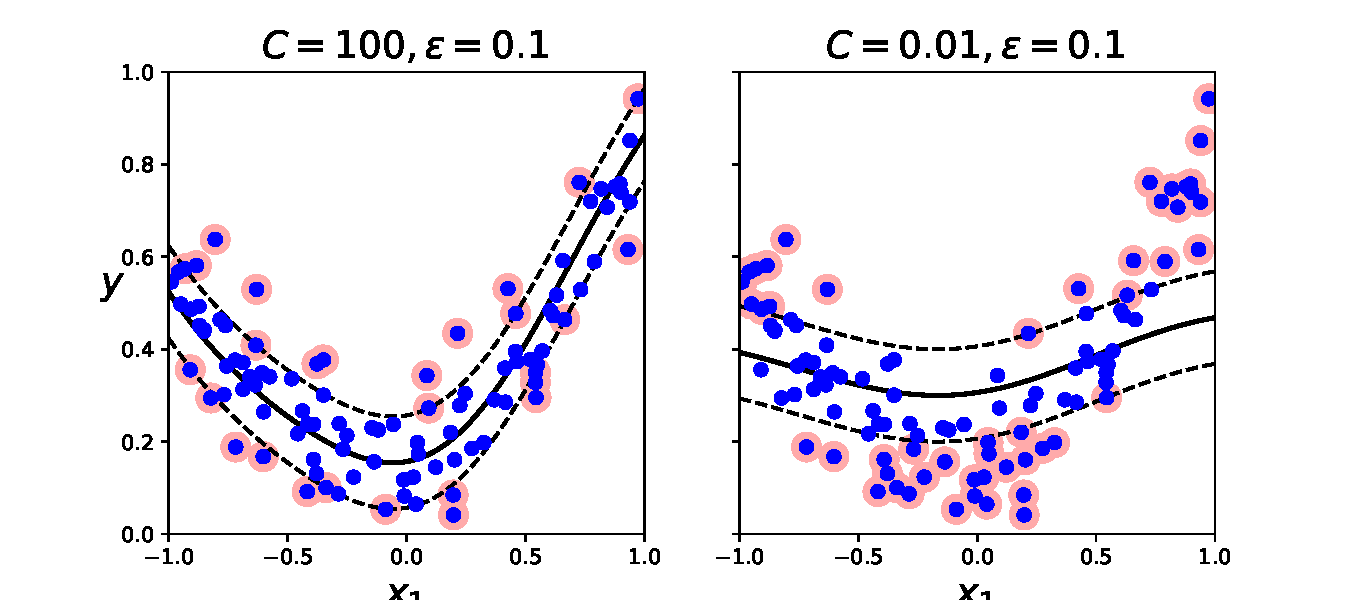
\includegraphics[width=0.25\textwidth]{svm_regression_e0p1.pdf}

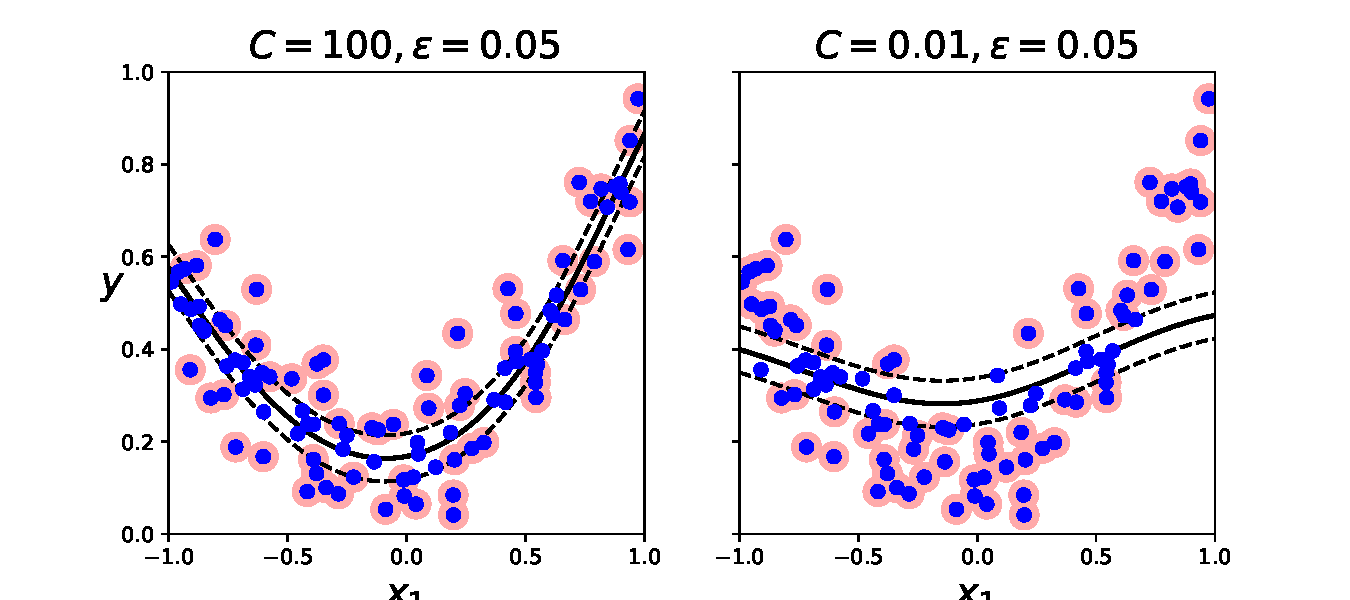
\includegraphics[width=0.25\textwidth]{svm_regression_e0p05.pdf}
\end{center}

\subsection{Kernel PCA}
\subsubsection*{Standard PCA}
Given a set of observations $x_i \in \mathbb{R}^{N}$, $i=1, \dots, m$, which are centered, $\sum_{i=1}^{m} x_i = 0$, PCA finds the principal axes by diagonalizing the covariance matrix:
\begin{equation*}
C = \frac{1}{m} \sum_{j=1}^{m} x_j x_j^{T}
\end{equation*}
$C$ is positive definite and can thus be diagonalized with nonnegative eigenvalues:
\begin{align*}
\lambda v & = C v = \frac{1}{m} \sum_{j=1}^{m} \langle x_j, v \rangle x_j 
\end{align*}

All solutions $v$ lie in the span of $x_1, \dots, x_m$, hence:
\begin{align*}
\lambda \langle x_i, v \rangle & = \langle x_i, C v \rangle
\end{align*}
for all $i = 1, \dots, m$.

\subsubsection*{Kernel PCA}
We are not interested in principal components in input space but of variables or features, which are nonlinearly related to the input variables.

\begin{align*}
\mathbf{\Phi} : \mathcal{X} & \rightarrow \mathcal{H} \\
x & \mapsto \mathbf{x} \coloneqq \mathbf{\Phi}(x)
\end{align*}

Again we are dealing with centered data. The covariance matrix takes the form:

\begin{equation*}
C = \frac{1}{m} \sum_{j=1}^{m} \mathbf{\Phi}(x_j) \mathbf{\Phi}(x_j)^{T}
\end{equation*}

All solutions $\mathbf{v}$ ($\lambda \mathbf{v} = \mathbf{C} \mathbf{v}$) lie in the span of $\mathbf{\Phi}(x_1), \dots, \mathbf{\Phi}(x_m)$. We may consider the set of equations:
\begin{align*}
\lambda \langle \mathbf{\Phi}(x_n), \mathbf{v} \rangle = \langle \mathbf{\Phi}(x_n), \mathbf{C}\mathbf{v} \rangle
\end{align*}
and there exists coefficients $\alpha_i$ such that:

\begin{align*}
\mathbf{v} = \sum_{i=1}^{m} \alpha_i \mathbf{\Phi}(x_i)
\end{align*}

Combining:

\begin{equation*}
m \lambda K \mathbf{\alpha} = K^2 \mathbf{\alpha}
\end{equation*}

We solve the dual eigenvalue problem:
\begin{equation*}
\boxed{m \lambda \mathbf{\alpha} = K \mathbf{\alpha}}
\end{equation*}
Let $\lambda_1 \geq \dots \geq \lambda_m$ denote the eigenvalues of $K$, and $\mathbf{\alpha}^1, \dots, \mathbf{\alpha}^m$ the corresponding complete set of eigenvectors. Let $x$ be a test point, with an image $\mathbf{\Phi}(x)$. Then:

\begin{align*}
\langle \mathbf{v}^n, \mathbf{\Phi}(x) \rangle = \sum_{i=1}^{m} \alpha_i^{n} \langle \mathbf{\Phi}(x_i), \mathbf{\Phi}(x) \rangle
\end{align*}

There is a way to compute the mean of the mapped observations in $\mathcal{H}$:
\begin{equation*}
\tilde{K}_{ij} = (K - 1_m K - K 1_m + 1_m K 1_m )_{ij}
\end{equation*}
using $(1_m)_{ij} \coloneq 1/m$ for all $i,j$.
\end{multicols}

\end{document}